\RequirePackage{plautopatch}

\documentclass[a4paper, 11pt]{ltjsarticle}


% マージン設定
\usepackage[top=20mm, bottom=20mm, left=20mm, right=20mm]{geometry}

% LuaLaTeX用日本語対応パッケージ
\usepackage{luatexja}
\usepackage{luatexja-fontspec}

% 必要なパッケージ
\usepackage{fontspec}
\usepackage{titlesec}
\usepackage{graphicx}
\usepackage{amsmath}
\usepackage{amssymb}
\usepackage[colorlinks=true, linkcolor=black, citecolor=black]{hyperref}
\usepackage{tocloft}
\usepackage{indentfirst}
\usepackage{tikz} % カスタム点線用
\usepackage{here}
\usepackage{subcaption}
\usepackage{bookmark}
\usepackage{booktabs}
\usepackage{multicol}
\usepackage{multirow}
\usepackage{flushend}
\usepackage{threeparttable}
\usepackage{enumitem}
\usepackage{url}
\usepackage{svg}

% 図:1のコロンを消す
\captionsetup{labelsep=space}

% 参考文献を上付きにする
\usepackage[super]{cite}
\renewcommand\citeform[1]{[#1]}

\setlength{\baselineskip}{14pt}
\setlength{\parindent}{1\zw}

\titleformat{\section}{\large\bfseries}{\thesection.}{1\zw}{}
\titleformat{\subsection}{\large\bfseries}{\thesubsection.}{1\zw}{}
\titleformat{\subsubsection}{\large\bfseries}{\thesubsubsection.}{1\zw}{}

\newcommand{\myref}[1]{\ref{#1}~(\alph{subtable})}

\setcounter{tocdepth}{3}
\makeatletter
\renewcommand{\numberline}[1]{#1.~}
\renewcommand{\cftsecleader}{\cftdotfill{\cftdotsep}}
\renewcommand{\cftsubsecleader}{\cftdotfill{\cftdotsep}}
\renewcommand{\cftsubsubsecleader}{\cftdotfill{\cftdotsep}}
\makeatother

\DeclareCaptionFont{designatedFont}{\fontsize{11pt}{14pt}\selectfont}
\captionsetup{font=designatedFont}

%---ここから中身---------------------------------------------------------------------------------------
\begin{document}
\fontsize{11pt}{14pt}\selectfont

%---表紙---------------------------------------------------------------------------------------
\thispagestyle{empty}
\begin{center}
\pagenumbering{gobble}  %ページ番号をカウントしない

\vspace*{40mm}
{\huge\noindent 災害時を想定したアドホックネットワーク}\\
\medskip
{\huge\noindent 構築手法の検討}\\
\vspace{\baselineskip}
{\huge\noindent\textbf{Study of Construction Methods for Ad-Hoc Network under Disaster}}\\
\vspace{120mm}

{\huge\noindent
2025年3月4日\\
東京都立産業技術高等専門学校\\
ものづくり工学科 情報通信工学コース \\
末廣 隼人\\
指導教員 髙﨑 和之    \\
}
\vspace{40mm}

\end{center}

%---目次------------------------------------------------------------------------------------------
\clearpage  %新しいページの追加
\thispagestyle{empty}
\tableofcontents  %目次の自動生成 目次をクリックするとその章,節に飛ぶことができる

%---はじめに---------------------------------------------------------------------------------------
\clearpage
\pagenumbering{arabic}
\section{はじめに}

% ・日本では地震をはじめ多くの自然災害が発生しており,災害時には通信ネットワークが使えなくなる可能性がある.
% そこで,アドホックネットワークを活用し地域限定ながら被災状況の把握や情報伝達を可能とする研究が行われている.\\
% ・本研究では,人口密度に応じた経路構築方法を考案し,その効果をシミュレーションを用いて検証した.\\
% ・近年,Bluetoothの開発が活発に行われており,従来のBluetooth Basic Rate/Enhanced Data Rate(BR/EDR)と比べて
% 大幅な省電力化が行われたBluetooth Low Energy(BLE)が発表された.そして,\\
% ・地震などの大きな災害が発生した際,従来の基地局を用いたネットワークへのアクセスの集中等により使用できなくなった場合,
% 新たなコミュニケーション環境の実現手段として,アドホックネットワークの研究が行われている.



%---理論---------------------------------------------------------------------------------------
\clearpage
\section{理論}
\subsection{アドホックネットワークについて} \label{about_ad-hoc}
アドホックネットワークとは,中央の管理者やルータ,アクセスポイントなどの既存のインフラストラクチャを介さずに,
端末(以下では,ノードと呼ぶ)同士が直接通信を行う一時的なネットワークのことである.
電波が届かず直接情報を交換できないノード同士の場合,基地局を経由せずに途中のノードが中継するマルチホップ通信により情報交換が可能になる.

これらを踏まえると,ノードさえあればどのようなエリアでも即席にネットワークを形成することができるためとても便利だが,
ノード移動に伴うネットワークトポロジや伝送品質の急激な変化,利用可能な無線周波数帯域の限界,バッテリ依存のノードの消費電力などの制約といった
厳しい条件がある.そのため,ルーティングやチャネルアクセスの制御,周波数帯域の有効活用,ノードの電力消費の節約等の多くの課題がある\cite{間瀬憲一2001アドホックネットワーク}.
図\ref{ad-hoc_model}にアドホックネットワークの使用イメージを示す.赤のノードが青のノードを経由し緑のノードに通信している図である.

アドホックネットワークに関する研究の歴史は長く,第1世代であるアドホックネットワーク"PRNET(Packet Radio Network)"
は1972年に米国の国防高等研究計画局によって開発され,軍事利用を目的とした研究のため実用化には至らなかった.
次に,第2世代となる"NTDR(Near-term Digital Radio)"も米国により軍事目的で研究が行われ,1980年代頃から実用化されている.
そして,第3世代となる"MANET(Mobile Ad hoc NETwork)"を含む現在のアドホックネットワーク技術はIEEE802.11やBluetoothなどの
近距離無線通信技術を活用し,民間でも使用できるアドホックネットワークが2000年頃から誕生した.同時期から災害時用ネットワークとして
の活用に期待が高まっていた.

\begin{figure}[H]
  \centering
  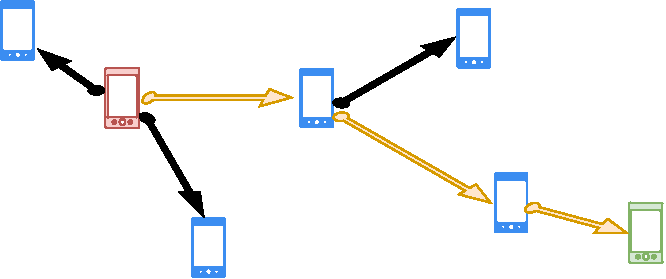
\includegraphics[width=85mm]{ad-hoc_model.pdf}
  \caption{アドホックネットワークのイメージ図}
  \label{ad-hoc_model}
\end{figure}

% \indent アドホックネットワークに関する研究の歴史が長く,1970年代初頭に軍事利用の観点から研究が開始された.1990年代半ばから世界的に研究が活発になり,1997年にはIETF(Internet Engineering Task Force)
% にMANET(Mobile Ad hoc NETwork)WGが発足され,ルーティングプロトコルを中心とした標準化の議論も開始された.

\subsection{ルーティングプロトコル}
ルーティングプロトコルは大きくリアクティブ型,プロアクティブ型,ハイブリッド型の3つに分類される(図\ref{routing_classification}).
次節にそれぞれの特徴と簡単な概略図を用いて紹介を行う.
\begin{figure}[H]
  \centering
  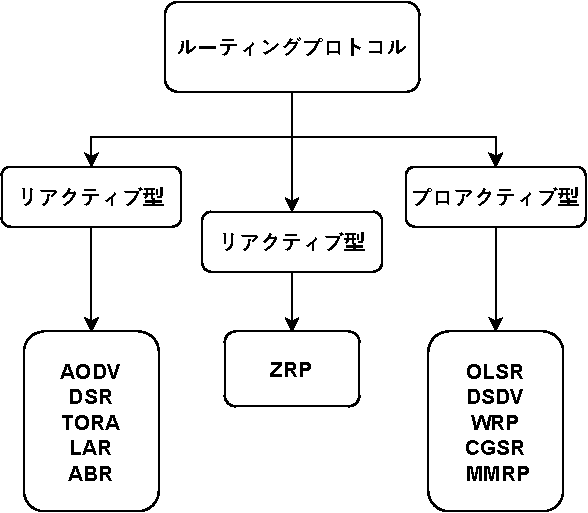
\includegraphics[width=85mm]{classification_of_routing.pdf}
  \caption{ルーティングテーブルの分類}
  \label{routing_classification}
\end{figure}

% \clearpage
\subsubsection{リアクティブ型}
あるノードが通信要求を行なった時にルーティングプロトコルに基づいて電波をフラッディングし,近隣のノードとその場で情報のやり取り行い経路生成を行う.
通信要求がなされた時に作成されるため,実際に通信が開始されるまでにラグが発生する.

このようにする理由として,アドホックネットーワークを構築するノードのほとんどが電池で駆動しているため,
むやみやたらに電波をフラッディングすると,すぐに電池が消費されてしまうからである.また,ノードは移動していることが多く,数分前の経路表が
無意味になってしまうことが多い.そのため,通信直前に経路表を生成することで電波のフラッディング回数を減らし,駆動時間の長時間化が行われる.
通信開始が遅くても良い環境で用いられている.代表的なプロトコルとして図\ref{routing_classification}よりAODV,DSR,TORA,LAR,ABRなどがある.

以下にリアクティブ型での動作イメージを図\ref{reactive}に示した.
\begin{enumerate}
  % (1)のように表示される
  \renewcommand{\labelenumi}{(\arabic{enumi})}
  \item \label{1} ノードA,ノードB,ノードCを設置し,各ノードには初期値として宛先が自身だけの経路表を保持している.
  \item \label{2} ノードA,C間で通信を行うことを想定し,自身のIDとノードCと通信したいという情報を載せてフラッディングを行う.
  \item \label{3} 情報を受け取ったノードBは送信先を記録し,宛先が誰かを確認し,自身でなければ自身のIDと宛先の情報を載せてフラッディングを行う.
  \item \label{4} (\ref{3})と同様に確認を行い,宛先が自身であるため,これまでの経路を逆順で経由してノードAに通信経路が作成されたことを伝える.
\end{enumerate}

% 縦に図を並ばせる
\begin{figure}[H]
  \centering
  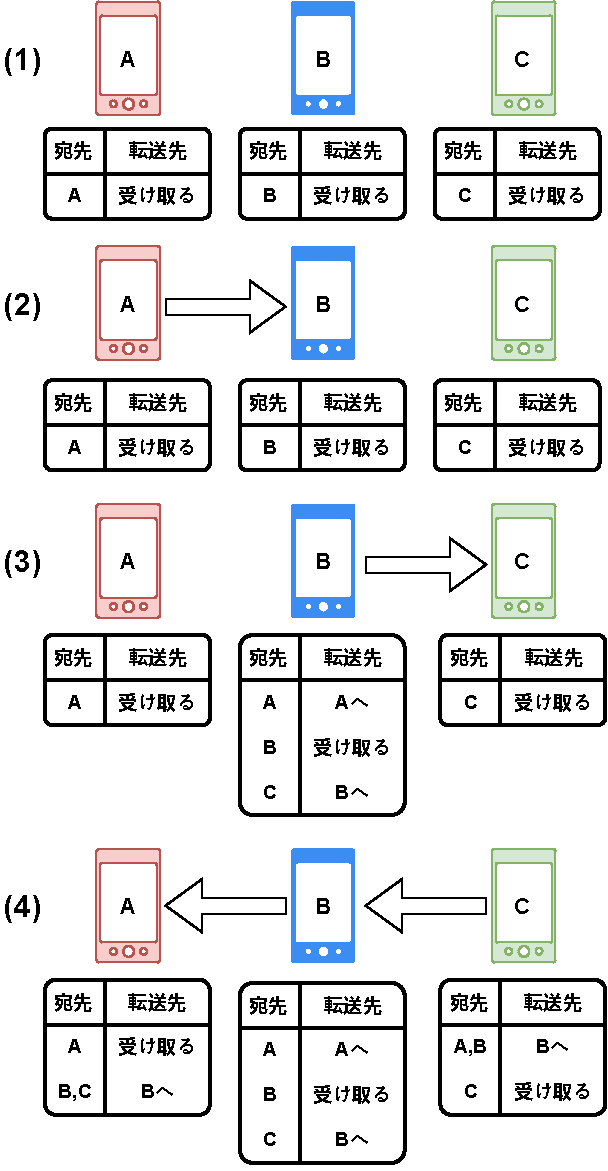
\includegraphics[width=75mm]{reactive_model.pdf}
  \caption{リアクティブ型の動作イメージ図}
  \label{reactive}
\end{figure}

\clearpage
\subsubsection{プロアクティブ型}
リアクティブ型では通信要求が発生してから経路表が作成されるのに対し,プロアクティブ型では近隣のノードと周期的に情報のやり取りを行い,
通信要求が発生したらすぐに通信を開始することができる.しかし,リアクティブ型と比べ頻繁に情報のやり取りを行うため,電池の消費が早い.
常に新鮮な経路表を保持しているためノードの入れ替わりが激しい環境では有効的である.代表的なプロトコルとして図\ref{routing_classification}
よりOLSR,DSDV,WRP,CGSR,MMRPなどがある.

以下にリアクティブ型での動作イメージを図\ref{proactive}に示した.各ノードは常に近隣のノードと情報をやり取りしているため,
通信の開始が早く,また,近隣のノードが接続が不可能になったとしても,すぐに新たな経路を生成することが可能であり安定した通信を行うことができる.
\begin{figure}[H]
  \centering
  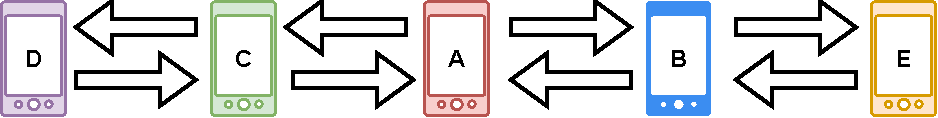
\includegraphics[width=80mm]{proactive_model.pdf}
  \caption{プロアクティブ型の動作イメージ図}
  \label{proactive}
\end{figure}

\subsubsection{ハイブリッド型}
リアクティブ型とプロアクティブ型の長所を組み合わせたプロトコルである.
代表的なプロトコルとして図\ref{routing_classification}よりZRP(Zone Routing Protocol)\cite{1574231874891177344}がある.

ZRPでは,ネットワークをゾーンと呼ばれる単位で分割し,ゾーン内にあるノードに対してはプロアクティブ型のルーティングプロトコルで近隣の情報同士でやり取りを行い,
ゾーン外にあるノードに対してはリアクティブ型のルーティングプロトコルで通信要求が発生した場合のみ動作しそのノードまでの経路を生成する.

メリットとして,ゾーン内では短距離通信の遅延が最小化され,ゾーン外では不要な情報のやり取りを減らすことが可能となる.
また,ネットワークが大規模になったとしても全ての経路情報を保持しなくて良いため効率的に運用することが可能である.
しかし,デメリットとして,ゾーン半径の設定が困難であることである.
ゾーン半径が小さい場合,遠距離通信が頻繁に発生してしまい,また,
ゾーン半径が大きい場合,ゾーン内に存在するノードが多数になり計算コストとメモリ消費が増大する可能性がある.

\subsection{アドホックネットワークの技術的課題}
\ref{about_ad-hoc}節で述べた課題のほかに,隠れ端末問題とさらし端末問題があり,
これらがアドホックネットワークが一般的に普及されていない原因の一つとも言える\cite{松井_進2012KJ00008330022}.
次項にそれぞれの問題について説明する.
\subsubsection{隠れ端末問題}
図\ref{hidden_problem}に隠れ端末問題を表した図を示す.図\ref{hidden_problem}では,
スマートフォンがノード,その周りにある円がノードからの通信距離を表している.
ノードBの円は見やすさの都合上省略している.

隠れ端末問題とは,ノードAとCがノードBに接続を行うとき,ノードA,Cは互いに通信可能距離外にあるため
互いの存在が隠れてしまい,ノードBが誰とも通信をしてないと判断してしまう.
そして,ノードA,Cが同時にデータをノードBに送信した場合,電波干渉やデータの衝突する問題が発生がある.

この問題により通信制御のスループット(処理能力)の低下が発生し,通信に遅延が生じる.
\begin{figure}[H]
  \centering
  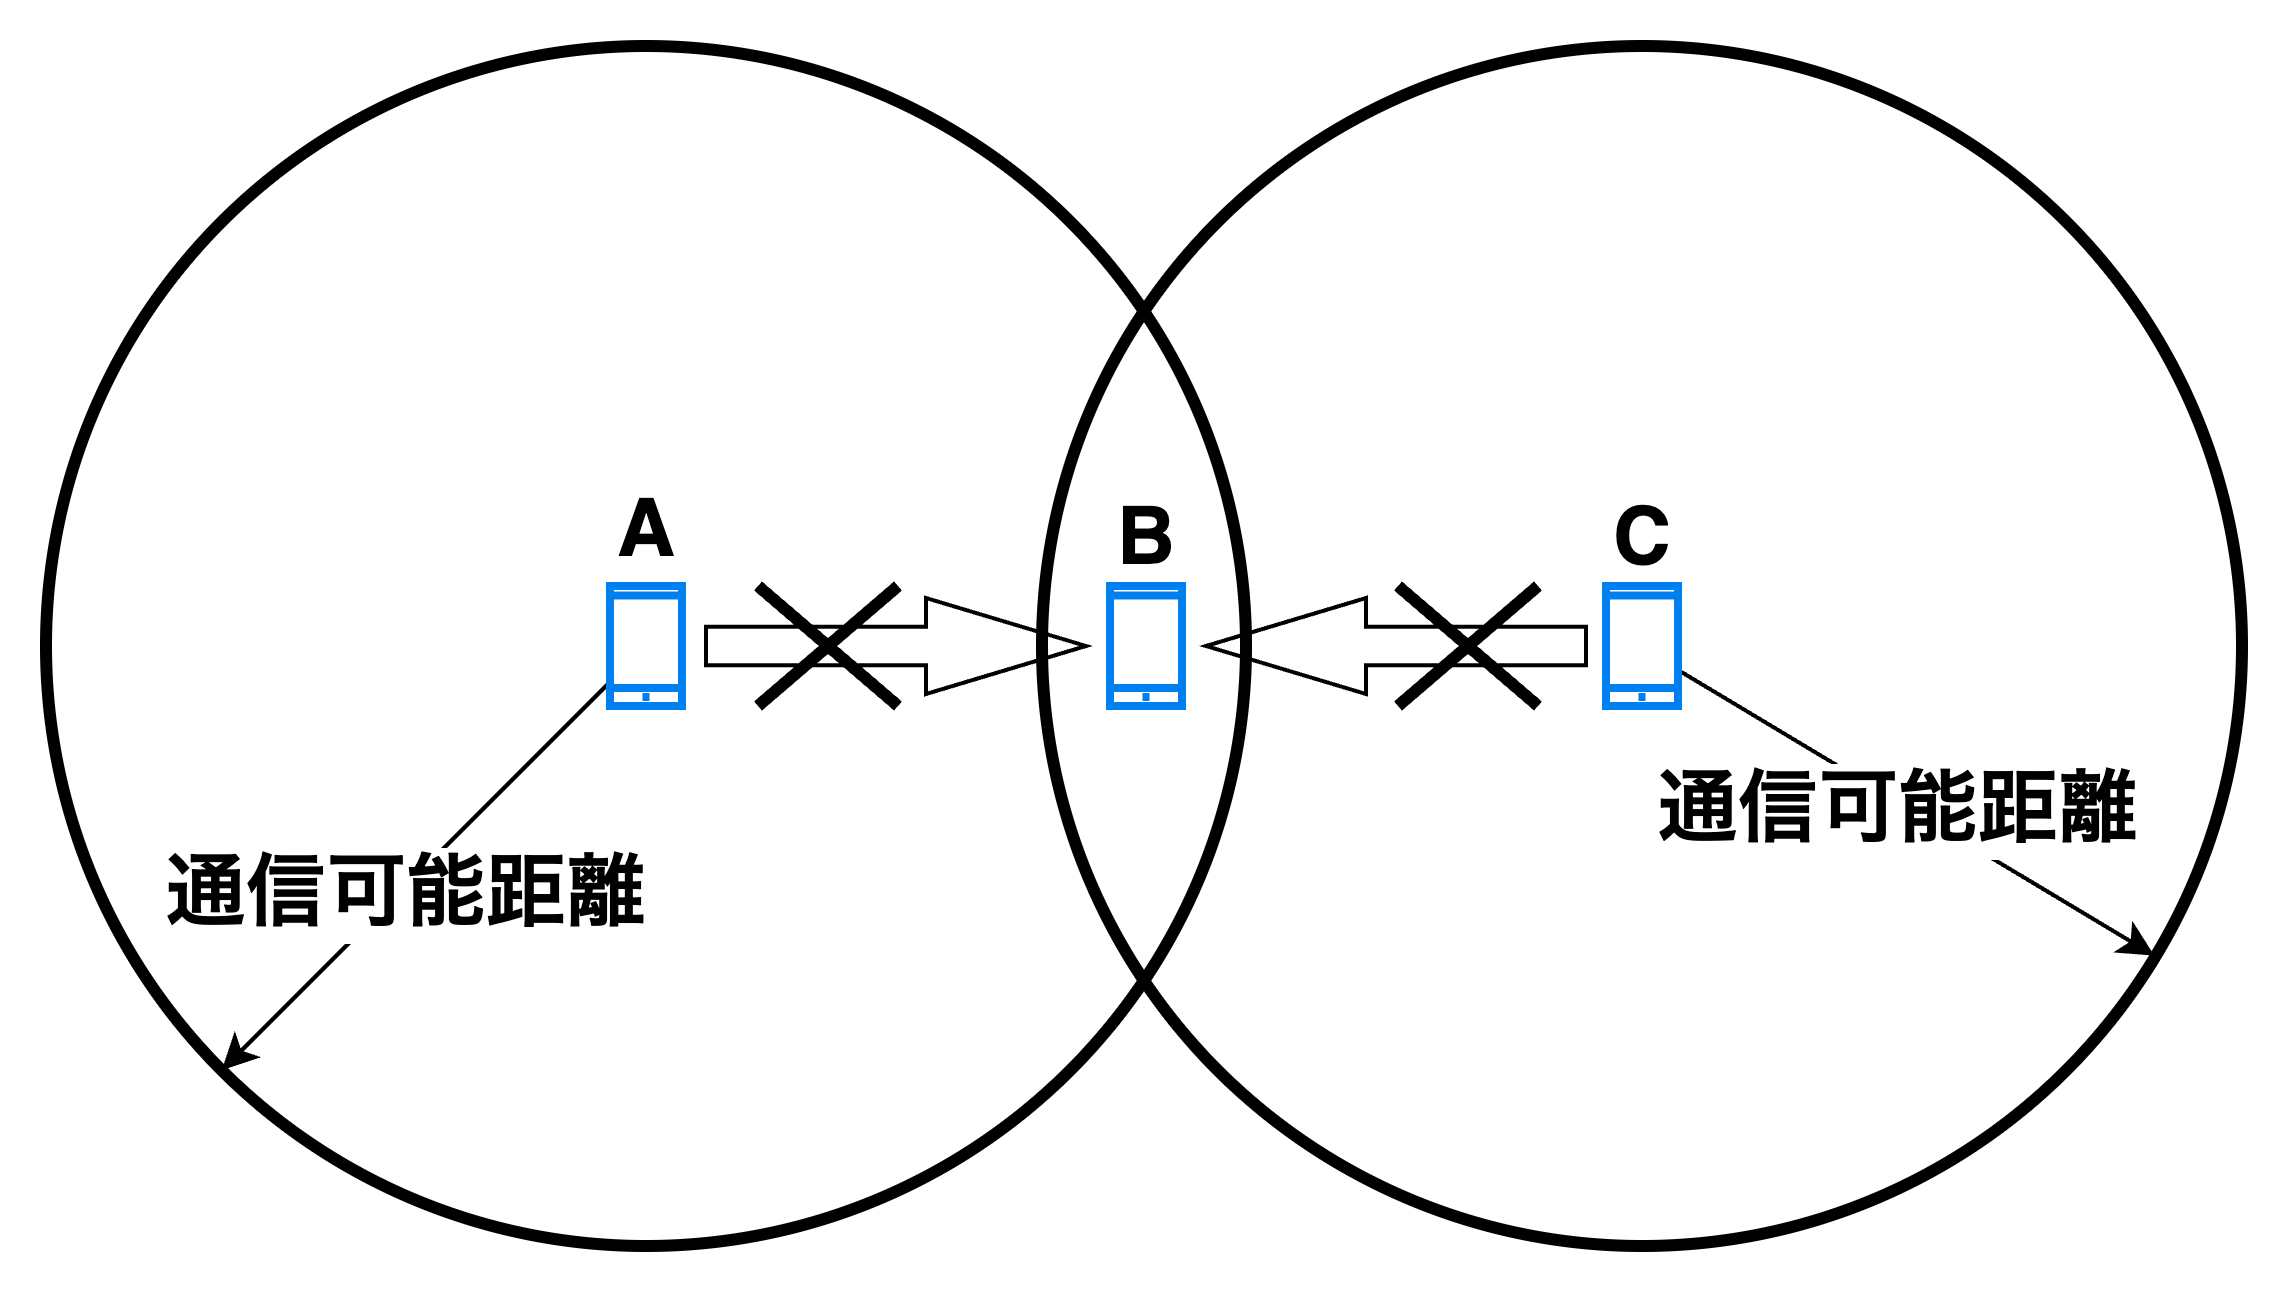
\includegraphics[width=100mm]{hidden_terminal_problem.png}
  \caption{隠れ端末問題}
  \label{hidden_problem}
\end{figure}

\subsubsection{さらし端末問題}
図\ref{exposed_problem}にさらし端末問題の図を示す.
図\ref{exposed_problem}で表されているスマートフォンや円は隠れ端末の場合と同様の意味である.

さらし端末問題とは,ノードA,Dが通信を行っているとき,通信可能距離内にいるノードBは
データを送信して衝突しないようにするために通信抑制が頻繁に行われる問題がある.これにより
伝送速度や通信品質の低下が発生してしまう.
\begin{figure}[H]
  \centering
  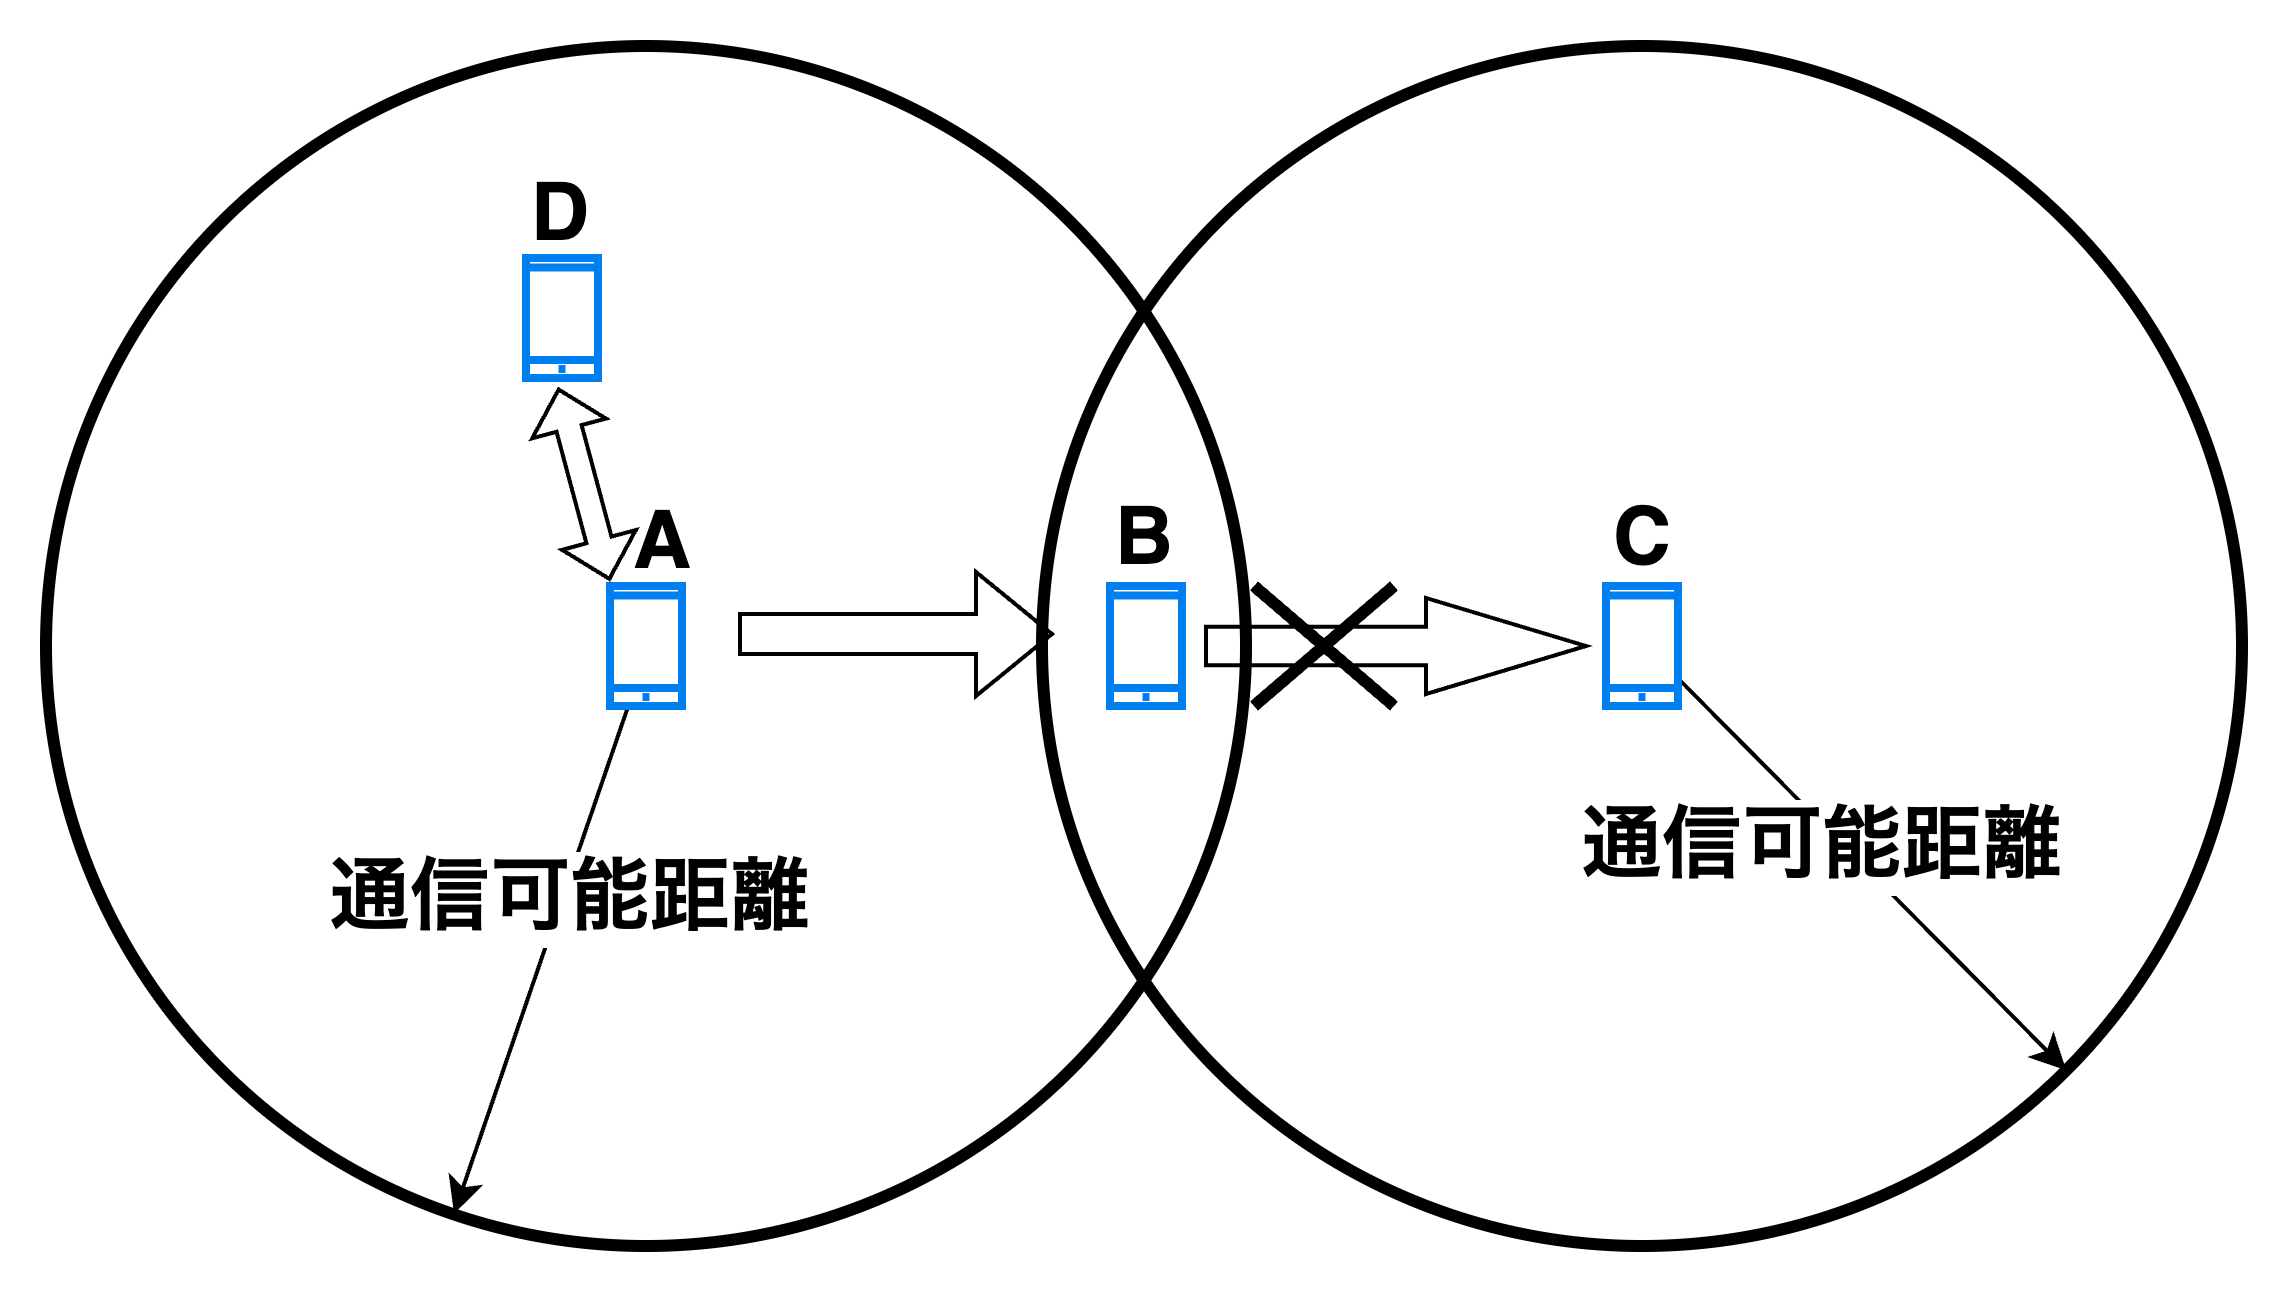
\includegraphics[width=100mm]{exposed_terminal_problem.png}
  \caption{さらし端末問題}
  \label{exposed_problem}
\end{figure}

% \clearpage
\subsection{Bluetooth}
Bluetoothは,2.4GHz帯の通信規格であり,数メートルから数十メートルほどの近距離通信機器などに用いられており,
IEEEの規格名はIEEE802.15.1である.
そして,現在のBluetoothには,ClassicとLow Energy(BLE)の2種類が存在し,異なる特徴を持つ.\\
表\ref{Bluetooth_characteristics}にそれぞれの特徴についてまとめた.

\subsubsection{Bluetooth Classic}
Bluetooth Classicは.デバイスと接続するときペアリング認証をし,再度同じ機器と接続するとき自動で接続され通信が行われる.
自動接続が行われ,情報のやり取りを頻繁に行うため消費電力が高くなっている.
また,通信トポロジはP2Pのスター型で,最大接続台数は7台となっている.
通信距離はClass1\textasciitilde3ように電波強度で分類され表2(b)のようになっている.

\subsubsection{Bluetooth Low Energy}
BLEは,最大転送速度が約1Mbpsで低速だが,低消費電力で駆動する.
Classicで行っていたペアリング認証を行わずに接続することが可能になった.また,
通信トポロジはスター型とメッシュ型の両方を持ち,接続台数が仕様上無限になりアドホックネットワークに向いている.
通信距離はデータ転送速度で異なり,表2(b)のようになっている.
現在では,Bluetooth 5.0以降では性能がより向上し,最大転送速度が2倍の2Mbpsになったり,通信距離が4倍の400mにもなりClassicにも
引けを取らないほどの性能となっている.また,方向探知やRSSI(受信信号強度)を用いた距離の推定を行う機能が搭載されている.

\begin{table}[h]
  \centering
  \caption{Bluetooth ClassicとBLEの特徴\cite{Bluetooth_official}}
  \begin{tabular}{c|c|c}
    \specialrule{1.5pt}{0pt}{0pt} % 上端の太線(1.5pt)
       & Bluetooth Classic & BLE \\
      \hline
      周波数帯 & \multicolumn{2}{|c}{2.4GHz (2.402 \textasciitilde 2.480GHz)} \\
      \hline
      チャネル利用 & \multicolumn{2}{|c}{周波数ホッピングスペクトラム拡散 (FHSS)}\\
      \hline
      チャネル数 & 1MHz間隔で79チャネル & 2MHz間隔で40チャネル \\
      \hline
      同時接続台数 & 最大7台 & 仕様上無限 \\
      \hline
      消費電力 & 1W & 0.01W \textasciitilde 0.5W \\
      \hline
      通信トポロジ & スター型 & スター型,メッシュ型 \\
      \hline
      主な用途 & マウス,イヤホンなど & IoTセンサ,スマートウォッチなど \\
      \specialrule{1.5pt}{0pt}{0pt} % 上端の太線(1.5pt)
  \end{tabular}
  \label{Bluetooth_characteristics}
\end{table}

% \begin{table}[h]
%   \centering
%   \caption{BLEの転送速度\cite{Bluetoothの通信距離}}
%   \begin{tabular}{c|c}
%     \specialrule{1.5pt}{0pt}{0pt} % 上端の太線(1.5pt)
%       バージョン & データレート \\
%       \hline
%       4.0 & 1Mbps \\
%       \hline
%       4.1 & 1Mbps \\
%       \hline
%       4.2 & 1Mbps \\
%       \hline
%       5 & 2Mbps,1Mbps,500kbps,125kbps \\
%       \specialrule{1.5pt}{0pt}{0pt} % 上端の太線(1.5pt)
%   \end{tabular}
%   \label{BLE_data_rate}
% \end{table}

\begin{table}[h]
  \centering
  \caption{通信距離\cite{Bluetoothの通信距離}}
  \begin{subtable}{0.49\textwidth} % (a) の表
    \centering
    \caption{Bluetooth Classicの場合}
    \begin{tabular}{c|l}
      \specialrule{1.5pt}{0pt}{0pt} % 上端の太線(1.5pt)
        Class 1 & 最大 100m (2.5mW超 \textasciitilde 100mW) \\
        \hline
        Class 2 & 最大 10m (1mW超 \textasciitilde 2.5mW) \\
        \hline
        Class 3 & 最大 1m (1mW) \\
        \specialrule{1.5pt}{0pt}{0pt} % 上端の太線(1.5pt)
    \end{tabular}
    \label{Classic_connecting_distance}
  \end{subtable}
  \hspace{-1.5cm}  % 表同士の間隔を狭くする
  \begin{subtable}{0.49\textwidth} % (b) の表
    \centering
    \caption{BLE(最大出力が100mW)の場合}
    \begin{tabular}{c|c}
      \specialrule{1.5pt}{0pt}{0pt} % 上端の太線(1.5pt)
        2Mbps & 最大 100m \\
        \hline
        1Mbps & 最大 100m \\
        \hline
        125kbps & 最大 400m \\
        \specialrule{1.5pt}{0pt}{0pt} % 上端の太線(1.5pt)
    \end{tabular}
    \label{BLE_connecting_distance}
  \end{subtable}
  \label{Bluetooth_connecting_distance}
\end{table}

% Bluetoothについての概要
% ・ワイヤレスオーディオ機器やなワイヤレス機器など短距離通信機器で用いられている
% ・Bluetooth Classic(BR(Basic Rate)/EDR(Enhanced Data Rate))とBLEの2種類ある
% ・Classicの特徴として,最大データ転送速度が高速(約3Mbps),常時接続が必要,消費電力が比較的大きい主にオーディオ機器やワイヤレス機器に用いられている.
% ・BLEの特徴として,最大データ転送速度は低速(約1Mbps),低消費電力,必要なときのみデータを送信する"アドバタイジング"方式,センサーデバイスやIoT機器に用いられている
% ・Bluetooth 5.0以降からはBLEの性能が向上し,最大データ転送速度が約2Mbpsに上昇,通信範囲が最大400m,Bluetooth Meshによるマルチデバイス接続の強化
% ・Bluetoothを用いて位置検出を行う研究が行われている\cite{勝野_恭治2002}
%---提案手法---------------------------------------------------------------------------------------
\clearpage
\section{提案手法}
経路探索を行うにあたって,日本の人口密度を参考にしてシミュレーションを行った.

%---結果---------------------------------------------------------------------------------------
\clearpage
\section{結果}

%---考察とまとめ---------------------------------------------------------------------------------------
\clearpage
\section{考察とまとめ}

%---参考文献---------------------------------------------------------------------------------------
\clearpage
\addcontentsline{toc}{section}{参考文献}
\bibliography{arxiv}
\bibliographystyle{junsrt}


\end{document}